\documentclass[a4paper,12pt]{article}
\usepackage[utf8]{inputenc}
\usepackage{amsmath, amssymb}
\usepackage{hyperref}
\usepackage{geometry} % Paket für Seitenränder
\usepackage{booktabs}
\usepackage[bottom]{footmisc}
\usepackage[ngerman]{babel}
\usepackage{graphicx}
\usepackage{xcolor} % Paket für Farben

\geometry{a4paper, top=25mm, bottom=40mm, left=35mm, right=35mm} % Seitenränder an Vorlage anpassen

% Dokument-Header
\title{Abgabe 1 für Computergestützte Methoden}
\author{\textcolor{red}{Gruppe 99\and 4107070 Jakob Bohn,\and 4371125 Nisa-Nur Civi,\and 4173169 Darleen Pastorik}} % author rot einfärben
\date{02.12.2024}

\begin{document}

\maketitle
\tableofcontents

\newpage

\section{Der zentrale Grenzwertsatz}
Der zentrale Grenzwertsatz (ZGS) ist ein fundamentales Resultat der Wahrscheinlichkeitstheorie, das die Verteilung von Summen unabhängiger, identisch verteilter (\textit{i.i.d.}) Zufallsvariablen (ZV) beschreibt. Er besagt, dass unter bestimmten Voraussetzungen die Summe einer großen Anzahl solcher ZV annähernd normalverteilt ist, unabhängig von der Verteilung der einzelnen ZV. Dies ist besonders nützlich, da die Normalverteilung gut untersucht und mathematisch handhabbar ist.

\subsection{Aussage}
Sei $X_1, X_2, \dots, X_n$ eine Folge von i.i.d. ZV mit dem Erwartungswert $\mu = \mathbb{E}(X_i)$ und der Varianz $\sigma^2 = \text{Var}(X_i)$, wobei $0 < \sigma^2 < \infty$ gilt. Dann konvergiert die standardisierte Summe $Z_n$ dieser ZV für $n \to \infty$ in Verteilung gegen eine Standardnormalverteilung:\footnote{Der zentrale Grenzwertsatz hat verschiedene Verallgemeinerungen.Eine davon ist der \textbf{Lindeberg-Feller-Zentrale-Grenzwertsatz} \cite[Seite 328]{klenke2013}, der schwächere Bedingungen an die Unabhängigkeit und die identische Verteilung der ZV stellt.}

\begin{equation}
\label{zn}
Z_n = \frac{\sum_{i=1}^n X_i - n\mu}{\sigma \sqrt{n}} \xrightarrow{d} \mathcal{N}(0, 1)
\end{equation}

Das bedeutet, dass für große $n$ die Summe der ZV näherungsweise normalverteilt ist mit Erwartungswert $n\mu$ und Varianz $n\sigma^2$:

\begin{equation}
\label{sumx}
 \sum_{i=1}^n X_i \sim \mathcal{N}(n\mu, n\sigma^2).   
\end{equation}

\subsection{Erklärung der Standardisierung}
Um die Summe der ZV in eine Standardnormalverteilung zu transformieren, subtrahiert man den Erwartungswert $n\mu$ und teilt durch die Standardabweichung $\sigma \sqrt{n}$. Dies führt zu der obigen Formel(\ref{zn}).Die Darstellung (\ref{sumx}) ist für $n \to \infty$ nicht wohldefiniert.

\subsection{Anwendungen}
Der ZGS wird in vielen Bereichen der Statistik und der Wahrscheinlichkeitstheorie angewendet. Typische Beispiele sind:
\begin{itemize}
    \item Schätzen von Populationsparametern in der Statistik.
    \item Hypothesentests in der medizinischen Forschung.
\end{itemize}

\newpage

\section{Bearbeitung zur Aufgabe 1}

\subsection{Datenverarbeitung}
Der Datensatz für unsere Gruppe enthält verschiedene Messwerte, die an der Fahrradverleihstation „West St \& Liberty St“ an jedem Tag im Jahr gemessen wurden. Dabei gibt es zu jedem Tag im Jahr Messwerte zu Temperatur, Niederschlag und Windgeschwindigkeit.

An den Daten kann man die Auslastung der Station zu verschiedenen Jahreszeiten oder zu bestimmten Wetterbedingungen vergleichen.

\subsubsection{Excel-Formel zur Abfrage von Maximalwerten}
Die folgende Formel wird auf einem neuen Arbeitsblatt in Excel angewendet:

\begin{verbatim}
=MAX(WENN('bike_sharing_data_(with_NAs)'!A:A=A2, 
          'bike_sharing_data_(with_NAs)'!J:J))
\end{verbatim}


\begin{figure}[h!]
    \centering
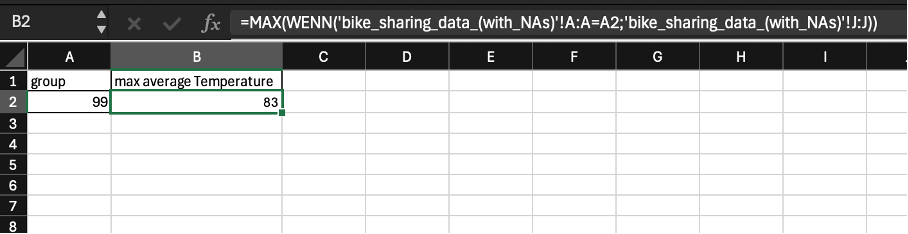
\includegraphics[width=\textwidth]{Comet_Snap_1.png}
    \caption{Excel-Ansicht.}
    \label{fig:example}
\end{figure}

Diese Formel bezieht sich auf das Arbeitsblatt „bike\_sharing\_data\_(with\_NAs)“ und gibt das Maximum der Spalte J aus. Es werden nur Werte berücksichtigt, bei denen der Wert in Spalte A der entsprechenden Zeile gleich dem Wert in Zelle A2 des neuen Arbeitsblatts ist.

So können die maximalen Durchschnittstemperaturen für verschiedene Gruppen abgefragt werden. Gibt man bei A2 den Wert „99“ ein, wird geprüft:
„Wenn in Spalte A der Wert 99 steht, dann wird der entsprechende Wert aus Spalte J in die MAX-Abfrage einbezogen.“

Das Maximum beträgt 83° für Gruppe 99.

\begin{figure}[h!]
    \centering
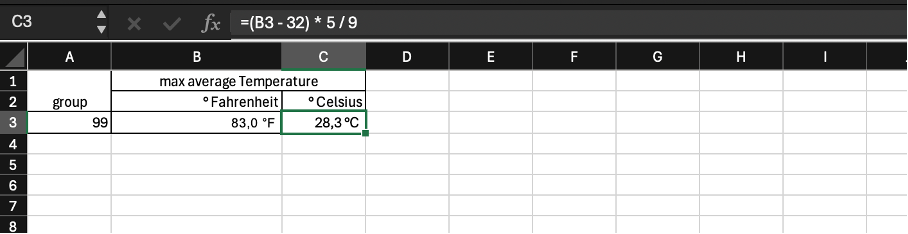
\includegraphics[width=\textwidth]{Comet_Snap_2.png}
    \caption{Excel-Ansicht 2.}
    \label{fig:example}
\end{figure}

Dieses Ergebnis ist in Grad Fahrenheit angegeben.


Um die Temperatur in Celsius umzuwandeln, kann folgende Formel angewendet werden:
\[
\text{Celsius} = (\text{Fahrenheit} - 32) \times \frac{5}{9}
\]
Nach der Umrechnung ergibt sich für die maximale Temperatur ein Wert von \( 28,3^\circ \mathrm{C} \), gemessen an der Station „West St \& Liberty St“.

\newpage

\subsection{Datenhaltung}
\subsubsection{Tabellenentwurf}
Schemata für die Tabellen \textit{Stationen}, \textit{Verleih} und \textit{Wetter}:

\begin{itemize}
    \item \textbf{Stationen}: (Id\#, Name)
    \item \textbf{Verleih}: (Id\#, StationId\#, Datum, Verleih\_anzahl)
    \item \textbf{Wetter}: (Id\#, Datum, temperatur\_mittel(in °C), niederschlag, windgeschwindigkeit)
\end{itemize}

Die Spalte \textit{StationId\#} verknüpft die Tabellen \textit{Stationen} und \textit{Verleih} als Fremdschlüssel.

\subsubsection{SQL-Befehle zur Tabellenerstellung}
Die Tabellen können mit den folgenden SQL-Befehlen erstellt werden:
\begin{verbatim}
CREATE TABLE Stationen (
    id INTEGER PRIMARY KEY,
    name TEXT NOT NULL
);

CREATE TABLE Verleih (
    id INTEGER PRIMARY KEY,
    station_id INTEGER,
    datum TEXT NOT NULL,
    verleih_anzahl INTEGER NOT NULL,
    FOREIGN KEY (station_id) REFERENCES Stationen(id)
);

CREATE TABLE Wetter (
    id INTEGER PRIMARY KEY,
    datum TEXT NOT NULL,
    temperatur_mittel FLOAT,
    niederschlag FLOAT,
    windgeschwindigkeit FLOAT
);
\end{verbatim}

\subsubsection{Importieren der Daten in SQLite}
Um die Daten aus vorbereiteten CSV-Dateien in SQLite zu importieren, können folgende Befehle verwendet werden:

\begin{verbatim}
.mode csv

.import "/Users/jakobbohn/stationen.csv" Stationen
.import "/Users/jakobbohn/stationen.csv" Verleih
.import "/Users/jakobbohn/stationen.csv" Wetter
\end{verbatim}

Der Dateipfad muss entsprechend angepasst werden. Je nach verwendetem CSV-Trennzeichen (Komma oder Semikolon) ist dieses ggf. auch zu ändern.

\subsubsection{SQL-Abfrage zur maximalen Temperatur}
Um die maximale mittlere Temperatur aus der Tabelle \textit{Wetter} abzufragen, kann folgende SQL-Abfrage verwendet werden:
\begin{verbatim}
SELECT MAX(temperatur_mittel) AS hoechste_mittlere_temperatur
FROM Wetter;
\end{verbatim}
Das Ergebnis gibt die höchste mittlere Temperatur im Datensatz aus.

\begin{figure}[h!]
    \centering
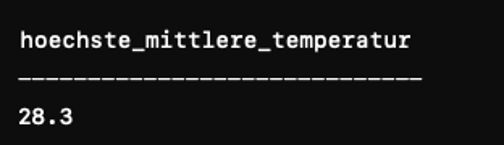
\includegraphics[width=\textwidth]{Comet_Snap_3.png}
    \caption{Ergebnisse der Abfrage.}
    \label{fig:example}
\end{figure}


\newpage

\begin{thebibliography}{9}
    \bibitem{klenke2013}
    Achim Klenke. \textit{Wahrscheinlichkeitstheorie.} Springer, 3. Auflage, 2013.
\end{thebibliography}


\end{document}
